\documentclass[UTF8]{ctexart}

\usepackage[linesnumbered,boxed,ruled,commentsnumbered]{algorithm2e}
\usepackage{bm}
\usepackage{graphicx}
\usepackage{float}
\usepackage[bookmarks=true]{hyperref}
\usepackage{amsmath}
\usepackage{geometry}


\geometry{a4paper,left=3cm,right=3cm,top=4cm,bottom=4cm}

\begin{document}
\title{$sin(x)$的数值计算与误差分析}
\author{陈昭熹 2017011552}
\maketitle
\tableofcontents
\newpage

\section{引言}
本文实现了通过数值方法求$sin(x)$,在一开头给出本文所实现的全部算法流程简述:
\begin{itemize}
    \item[\textbf{级数逼近法}] 使用级数逼近$sin(x)$
    \item[\textbf{常微分方程法}]通过三角函数关系$\sin^2{x}+\cos^2{x}=1$,利用改进欧拉法求解关于$sin(x)$的微分方程。
    \item[\textbf{微小增量法}] 利用三角函数和角公式$sin(x+h)=sin(x)cos(h)+cos(x)sin(h)$,利用小增量累加来求解$sin(x)$。
\end{itemize}

后面章节中,逐节介绍各个算法的原理、误差分析、算法流程以及计算代价和收敛速度。第5节介绍算法利用C++的程序实现以及具体流程(以流程图形式给出),第6节展示一些实验结果并做总结。

\section{级数逼近法}

本节介绍利用级数逼近法计算$sin(x)$的任意精度算法。

\subsection{算法原理}

众所周知,根据$sinx$在$x_0=0$的邻域$(-h+x_0,h+x_0)$内的Taylor展开式,有如下式子成立:
\begin{equation}
    \sin{x} = \sum^\infty_{n=0} \frac{(-1)^nx^{2n+1}}{(2n+1)!}=x-\frac{x^3}{3!}+\frac{x^5}{5!}-\frac{x^7}{7!} \dots + \frac{x^{2n+1}}{(2n+1)!}+R_k(x)
\end{equation}

注意这里写了余项形式(为了表示方便,将展开阶次表示为k,有k=2n+1),因此可以精确取等。若存在正实数$M_k$使得区间$(-h,h)$上的任意x均有$|f^{(k+1)}(x)|\leq M_k$,则上式中余项估计为:
\begin{equation}
    |R_k(x)|\leq M_k \frac{h^{k+1}}{(k+1)!}
\end{equation}

这样的一个上界估计对$x_0$的邻域内的任意x均成立,是一个一致估计。利用式(1),只需要控制展开的阶数,就可以实现任意精度的$sinx$数值计算。

需要注意的是,这里有一个前提,即上述展开是在原点处的邻域内进行的,因此需要\textbf{通过$sinx$的周期性,尽可能将自变量x变换到原点附近},避免不满足邻域条件导致误差过大。


\subsection{误差分析}

\subsubsection{方法误差}

上一小节已给出级数逼近法的余项形式,这里进行误差分析。由$sinx$无穷阶光滑特性及周期性可以得到$$M_k \leq 1$$
因此有方法误差
\begin{equation}
    |R_k(x)| \leq \frac{h^{k+1}}{(k+1)!}
\end{equation}

事实上,这里可以通过微分中值定理得到一个精确地误差表达形式,即用$\sin^{(k+1)}{(\xi)}$来代替$M_k$,但是这样无法进行量化分析,因此进行一定的放缩,给出上界。式子中的$h$即实现时候将所有x值利用周期性映射到原点附近的区间$(-h,h)$,一般为$(-\pi/2,\pi/2)$。依据这个上界,可以通过控制多项式展开的阶数$k$来控制方法误差,在理论上达到任意精度。

值得注意的是对于偶数位精度要求,本方法具备天然高一阶的精度(即k=2n+1)。

\subsubsection{舍入误差}

假设每个阶次的计算均精确到$d$位小数,则存储带来的舍入误差为:$$\delta_0 = \frac{1}{2}\times 10^{-d}$$

则求和带来的舍入误差为:
\begin{equation}
    \delta = (n+1) \cdot \delta_0 = (n+1) \times \frac{1}{2}\times 10^{-d}
\end{equation}

\subsubsection{总误差}

因此总误差
\begin{equation}
    A = |R_k(x)| + \delta \leq \frac{h^{k+1}}{(k+1)!} + \frac{n+1}{2} \times 10^{-d}
\end{equation}

\subsection{计算代价与收敛速度}
计算代价方面,由于使用递归算法,因此计算阶乘和幂级数的代价均为$O(k)$,而求和的代价也为$O(k)$,因此总体来说还是一个线性的计算速度$O(3k)$。由于余项收敛是泰勒展开成立的条件,因此无需担心收敛速度慢的问题,因为阶乘的增长速度远比幂级数快得多,严格计算则需要归约$\frac{h^{k+1}}{(k+1)!}$,这个数学问题显然比本问题复杂得多。值得注意的是,当$k+1>h$时,$|R_k(x)|$开始以$O(a^{k}),0<a<1$的速度收敛,因此整体的收敛速度仍是常数$O(h)$。这也从另一个侧面说明,在计算过程中将自变量x变换到较小的原点邻域内的巨大作用,若使用原始的x进行计算,会使得h值过大,导致在相同精度要求下,收敛速度急剧变慢,计算代价升高。
\section{常微分方程法}

本节介绍利用常微分方程法计算$sinx$的任意精度算法。

\subsection{算法原理}
利用$\frac{dsin(x)}{dx}=cos(x)$,可以得到下面的常微分方程组:
\begin{equation}
    \frac{d}{dx}\left(
    \begin{matrix}
            cosx \\
            sinx
        \end{matrix}
    \right)=\left(
    \begin{matrix}
            -sinx \\
            cosx
        \end{matrix}
    \right)
\end{equation}

尽管需要计算$sinx$的数值,但还是存在可以加以利用的先验知识——$sin0 = 0$,利用这一点的值作为初始条件,采用改进欧拉法即可求解这一微分方程组在给定点的解。

改进欧拉法分为两个步骤:预测和矫正,若选择的区间间隔为$h$,则可以表达为下式:

\begin{equation}
    \begin{cases}
        \bar{y}_{n+1}=y_n+hf(x_n,y_n) \\
        y_{n+1}=y_n+\frac{h}{2}[f(x_n,y_n)+f(x_{n+1},\bar{y}_{n+1})]
    \end{cases}
\end{equation}

对于本问题,有初始条件:
\begin{equation}
    x_0=0,cos(x_0)=1,sin(x_0)=0
\end{equation}

虽然改进欧拉法只给出了求解一个方程的步骤,注意到本问题的微分方程组有良好的相关性,可以“串联”在一起,就可以较好的将改进欧拉法推广到上面。为表达方便将$cos(x)$简写为$c$,将$sin(x)$简写为$s$,下标表示与$x$的含义相同,则具体做法如下:
\begin{equation}
    \begin{aligned}
        \bar{c}_{n+1} &= c_n + h\times(-s_n)\\
        \bar{s}_{n+1} &= s_n + h\times c_n\\
        c_{n+1} &= c_n + \frac{h}{2}[(-s_n)+(-\bar{s}_{n+1})]\\
        s_{n+1} &= s_n + \frac{h}{2}(c_n+\bar{c}_{n+1})
    \end{aligned}
\end{equation}

\subsection{误差分析}

\subsubsection{方法误差}
方法误差可以从两部分来分析,一部分来源于预测,一部分来源于校正。

首先分析预测带来的局部截断误差,设$y_n = y(x_n)$,分析$\bar{y}_{n+1} - y(x_{n+1})$。由欧拉公式预测法的公式:
\begin{equation}
    \bar{y}_{n+1} = y_n + hf(x_n,y_n)
\end{equation}

对于精确值$y(x_{n+1})$进行泰勒展开有下式:
\begin{equation}
    y(x_{n+1}) = y(x_n) + hy^{(1)}(x_n) + \frac{h^2}{2}y^{(2)}(x_n)+\dots
\end{equation}

根据微分方程约束条件$f(x_n,y_n) = y'(x_n)$,(10)与(11)式相减后再求导可得:
\begin{equation}
    \bar{y}'_{n+1} - y'(x_{n+1}) \doteq \frac{h^2}{2}\frac{\partial f}{\partial y} \Bigg|_{x=x_n} \cdot y^{(3)}(x_n)
\end{equation}

上式可以作为预测一步带来的局部截断误差,代入校正一步进行分析。对于校正一步,分析$y(x_{n+1}) - y_{n+1}$。根据校正公式:
\begin{equation}
    \begin{aligned}
        y_{n+1} &= y_n + \frac{h}{2}[f(x_n,y_n)+f(x_{n+1},\bar{y}_{n+1})]\\
        &= y_n + \frac{h}{2}[y'(x_n)+\bar{y}'_{n+1}] \\
        &= y_n + \frac{h}{2}[y'(x_n)+y'(x_{n+1})+\frac{h^2}{2}y^{(3)}(x_n)]\\
        &= y_n + \frac{h}{2}[y'(x_n)+y'(x_n) + hy^{(2)}(x_n) + \frac{h^2}{2}y^{(3)}(x_n)+\dots + \frac{h^2}{2}\frac{\partial f}{\partial y} \Bigg|_{x=x_n} \cdot y^{(3)}(x_n)]
    \end{aligned}
\end{equation}

对于精确值$y(x_{n+1})$进行泰勒展开有下式:
\begin{equation}
    y(x_{n+1}) = y_n + hy'(x_n) + \frac{h^2}{2}y^{(2)}(x_n) + \frac{h^3}{3!}y^{(3)}(x_n) + \dots
\end{equation}

同理,将(13)与(14)相减,可以得到同时考虑预测和校正的局部截断误差:
\begin{equation}
    y(x_{n+1}) - y_{n+1} = (-\frac{h^3}{12} - \frac{h^3}{4}\frac{\partial f}{\partial y} \Bigg|_{x=x_n})\cdot y^{(3)}(x_n) \doteq O(h^3)
\end{equation}

上面的分析是针对一阶微分方程,而本问题相当于两个一阶微分方程,每次局部截断误差将叠加两次,但是这并不妨碍误差分析,只不过本问题中局部截断误差的具体系数需要在上面分析的基础上翻倍,但从归约角度上来看,局部截断误差仍是$O(h^3)$,因此累计起来整体算法仍是二阶精度:
\begin{equation}
    \begin{aligned}
    \Delta_{n+1} &\doteq \Delta_n + h\cdot \frac{\partial f}{\partial y}\Delta_n + (-\frac{h^3}{12} - \frac{h^3}{4}\frac{\partial f}{\partial y} \Bigg|_{x=x_n})\cdot y^{(3)}(x_n)\\
    &\doteq\Delta_n + (-\frac{h^3}{12} - \frac{h^3}{4}\frac{\partial f}{\partial y} \Bigg|_{x=x_n})\cdot y^{(3)}(x_n)\\
    &\doteq O(h^2)
    \end{aligned}
\end{equation}


\subsubsection{舍入误差}

事实上,为了实现起来较为方便,在代码中使用了如下的计算逻辑:
\begin{equation}
    \begin{cases}
        y_p = y_n + hf(x_n,y_n)\\
        y_q = y_n + hf(x_n+h,y_p)\\
        y_{n+1} = \frac{1}{2}(y_p+y_q)
    \end{cases}
\end{equation}

假设每次计算均精确到$d$位小数,则存储带来的舍入误差为:$$\delta_0 = \frac{1}{2}\times 10^{-d}$$

则每一步迭代均涉及3x2=6次加法,因此迭代n步之后加法带来的累计舍入误差:
\begin{equation}
    \delta = 6n\delta_0 = 6n\times \frac{1}{2}\times 10^{-d}    
\end{equation}


\subsubsection{总误差}

因此总误差可以表示为:
\begin{equation}
    A = \Delta_{n+1} + \delta
\end{equation}

其中具体表达式在此不做展开,上文中(16)和(18)均已明确表示。



\subsection{计算代价与收敛速度}
给定精度$d$,则根据上面的误差分析可知,本方法是一个二阶方法,只需要$O(\frac{1}{\sqrt{d}})$的时间就可以收敛。对于计算代价,每次迭代均为常数时间,因此计算代价与收敛速度应当同阶。

\section{微小增量法}

说实在的,这个方法笔者也不知道应该取个什么名字。起初是受到了快速离散傅里叶变换的实现的启发,注意到三角函数一个十分简单的和角公式:
\begin{equation}
    \begin{cases}
        sin(x_n+h) = sin(x_n){cos}(h)+cos(x_n){sin}(h)\\
        cos(x_n+h) = cos(x_n){cos}(h) - sin(x_n){sin}(h)
    \end{cases}
\end{equation}

实际上DFT的计算机实现中,相应三角函数的值就是通过先前一点和增量来进行计算的。使用上式,只需要确定小增量$cos(h),sin(h)$,就可以通过累加的方式计算出$sin(x+nh)$的数值解。

\subsection{算法原理}

算法的前提建立在本文前面提到过的,已经将x通过三角函数周期性变换到$[0,\frac{\pi}{2}]$上。此时需要确定小增量$h$。类似于数值积分的方法,可以令$h=\frac{x-0}{n}$,这样就可以通过迭代次数来控制算法精度。

注意到这个方法有一个天然的优势,那就是由于$h$是小量,非常靠近原点,因此很好的满足了三角函数在原点泰勒展开的邻域要求,使得通过泰勒展开来近似求取$cos(h),sin(h)$将带来很小的误差。注意到这一点,本方法直接使用三阶的泰勒展开来近似微小增量:
\begin{equation}
    \bar{sin}(h) = h - \frac{h^3}{6} + O(h^3) \doteq  h - \frac{h^3}{6}
\end{equation}

事实上,对于$\bar{cos}(h)$也可以用相同的近似方法,但是考虑到在原点附近余弦值接近1,这会导致其实际表征信息的有效数字位数较少(被前面的.9999所吃掉),在不同的区间长度$h$下,可能会出现精度损失问题。因此在实现过程中,将小量$\bar{cos}(h)$通过二倍角公式定义为$sin(h)$型,来避免精度损失:
\begin{equation}
    \bar{cos}(h) = 1-2sin^2(\frac{h}{2})
\end{equation}

得到了初始条件后,就可以通过式(20)来迭代地计算,最终得到$sin(x)$的数值。

\subsection{误差分析}

\subsubsection{方法误差}

本方法的另一优点是其迭代方式定义清晰,且误差项被分离出来,十分便于进行精确地误差分析。

首先考虑局部截断误差,即假设$sin(x_n),cos(x_n)$是精确的,分析$sin(x_{n+1})$的误差。
这里不仿照求解常微分方程时的误差分析,将精确值和估计值分别进行泰勒展开,原因有二。一是迭代式中非线性的三角函数关系,因此不便于利用级数进行误差分析;二是误差项已经在初始条件中明确的给出,是一个可以控制的常量。

由初始条件的展开阶数可知,每一次的微小增量误差为:
\begin{equation}
    \delta_0 = \frac{h^3}{3!}sin^{(3)}(\xi) \leq \frac{h^3}{6}
\end{equation}

因此(cosx使用二倍角公式进行定义变换,需要通过求偏导来得到其误差):
\begin{equation}
    \begin{cases}
        \bar{cos}(h) = cos(h) - 4\times{(\frac{1}{2})}^3\delta_0 = cos(h) - \frac{\delta_0}{2}\\
        \bar{sin}(h) = sin(h) - \delta_0
    \end{cases}
\end{equation}

将(24)带入到(20)中,得到:
\begin{equation}
    \begin{aligned}
        \bar{sin}(x_{n+1}) &= sin(x_n)[cos(h)-\frac{\delta_0}{2}] + cos(x_n)[sin(h) - \delta_0]\\
        &=sin(x_n)cos(h)+cos(x_n)sin(h) - \frac{\delta_0}{2}sin(x_n)-\delta_0 cos(x_n)\\
        &=sin(x_{n+1}) - [\frac{\delta_0}{2}sin(x_n)+\delta_0 cos(x_n)]\\
    \end{aligned}
\end{equation}

\begin{equation}
    \Rightarrow \delta_s(n+1) = \bar{sin}(x_{n+1})-sin(x_{n+1}) = - [\frac{\delta_0}{2}sin(x_n)+\delta_0 cos(x_n)]
\end{equation}

类似地:
\begin{equation}
    \begin{aligned}
        \bar{cos}(x_{n+1}) &= cos(x_n)[cos(h)-\frac{\delta_0}{2}] - sin(x_n)[sin(h) - \delta_0]\\
        &= cos(x_{n+1}) + \delta_0sin(x_n)-\frac{\delta_0}{2}cos(x_n)
    \end{aligned}
\end{equation}

\begin{equation}
    \Rightarrow \delta_c(n+1) = \bar{cos}(x_{n+1})-cos(x_{n+1}) = \delta_0sin(x_n)-\frac{\delta_0}{2}cos(x_n)
\end{equation}

为了便于分析进行一定放缩:
\begin{equation}
    \begin{cases}
        |\delta_s(n+1)| \leq \frac{3}{2}\delta_0 \\
        |\delta_c(n+1)| \leq |\delta_0 sin(x_n)| + |\frac{\delta_0}{2}cos(x_n)| \leq \frac{3}{2}\delta_0
    \end{cases}
\end{equation}

利用(29)两个局部截断误差递推式,可以推导出累计误差,过程如下:
\begin{equation}
    \begin{aligned}
        \Delta_s(n+1) &= \Delta_s(n) + \delta_s(n+1) \\
        \Rightarrow \Delta_s(n+1) - \Delta_s(n) &= \delta_s(n+1)\\
        &\dots\\
        \Delta_s(1) - \Delta_s(0) &= \delta_s(1)\\
    \end{aligned}
\end{equation}

经过叠加法可以得到累计误差:
\begin{equation}
    \begin{aligned}
        \Delta_s(n+1) &= \Delta_s(0) + \sum_{i=0}^{n}\delta_s(i+1)\\
        &= \sum_{i=0}^{n+1}\delta_s(i)\\
        &\leq \frac{3}{2}(n+1)\delta_0 \\
        &\leq \frac{3}{2}(n+1)\frac{h^3}{6}\\
        &= \frac{1}{4}(n+1)\frac{x-0}{n} \cdot h^2
        \doteq O(h^2)
    \end{aligned}
\end{equation}

可以看出,其仍是一个二阶精度算法,与上一节的方法一致。实现过程中,可以通过控制区间分割长度$h$来控制精度。或者通过调整微小增量的展开阶数,来将算法精度的阶数进行质的改变。可以说,这一点是比本算法的一个亮点。

\subsubsection{舍入误差}

假设微小增量的存储精确到$d_0$位小数,则后面每一步的迭代计算都会携带这个舍入误差。$$\epsilon_0 = \frac{1}{2}\times 10^{-d_0}$$

在后续计算中,假设每次计算均精确到$d$位小数,则其存储带来的舍入误差为:$$\epsilon_s = \frac{1}{2}\times 10^{-d}$$

舍去求偏导的过程,将三角函数均放缩到1,故总体舍入误差:
\begin{equation}
    \epsilon < (2\epsilon_0+\epsilon_s)n
\end{equation}

\subsubsection{总误差}

因此总误差可以表示为:
\begin{equation}
    A = \Delta_s(n+1) +\epsilon
\end{equation}

其中具体表达式在此不做展开,上文中(31)和(32)均已给出。


\subsection{计算代价与收敛速度}

由于其累计精度以及控制精度方法均和上一节的常微分方程法类似,因此其收敛速度和计算时间代价是类似的。但是值得注意的是,由于其控制精度入口可以通过控制微小增量的展开阶数来直接提高算法的精度阶数,从而大幅提高收敛速度,而且这样做的代价是极小的。
\section{算法流程与实现}

询问过助教,本次大作业不需要实现UI界面,因此就没有大费工夫做一个美观的GUI界面。在命令行中运行main文件,根据提示输入自变量x,并选择求解算法后,可以获得相应结果。程序可以一直运行直至用户输入回车结束。

其中求解算法的流程图如下所示,按照助教要求默认精度保留小数点后四位:
\begin{figure}[H]
    \centering
    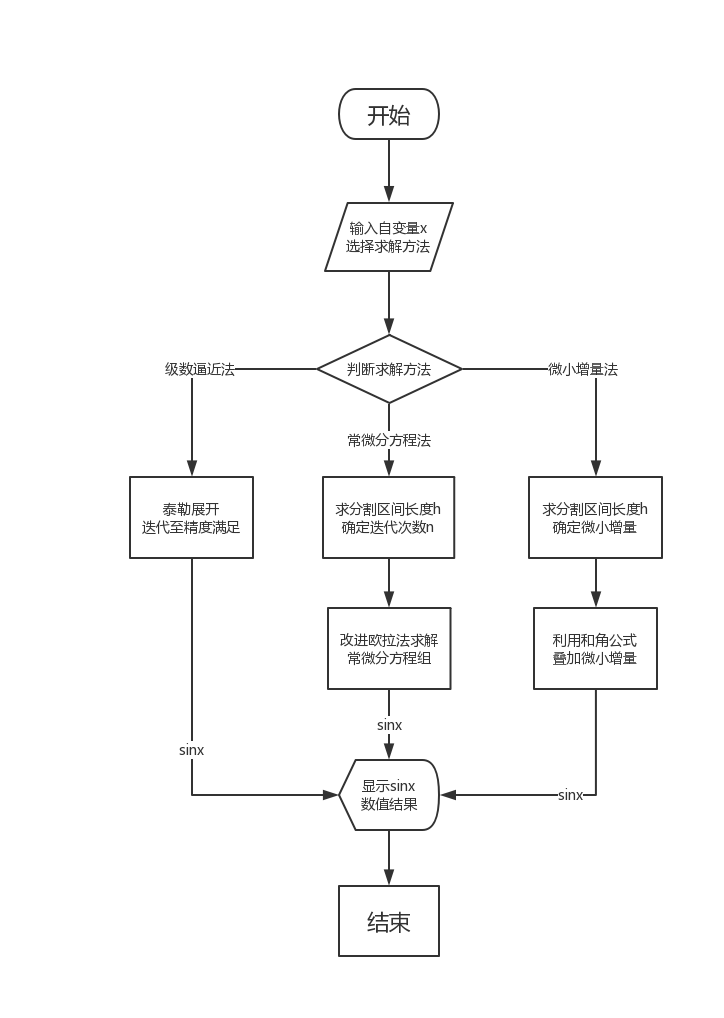
\includegraphics[scale=0.4]{images/procedure.png}
    \caption{求解sinx数值解算法流程图}
\end{figure}

\section{结果与总结}

\subsection{与C++标准Math库结果对比}

\subsection{总结和体会}
通过本次实验,我温习了课上讲过的多种数值分析算法:Taylor级数、函数逼近、求解常微分方程等算法。在误差分析的过程中,我更加熟悉了方法误差、舍入误差的分析方法。
本次大作业中,我的完成方法是首先设计算法,其次进行充分的误差分析,再通过误差分析的结果来完成算法的实现。这不同于以往我的习惯,本次先分析后实现的流程确实让我体会深刻,能够对于将要实现的东西更加明确,在实现过程中也少踩了很多坑,极大地加快了进度。

对于方法的创新设计,我曾经想到过利用欧拉公式$e^{ix} = cos(x)+isin(x)$来进行求解,但查阅了很多资料也没想好如何处理复数域问题及其误差分析。也曾经想到过利用反三角函数$arcsin(x)$,由于它是可以利用数值积分$\int\frac{1}{\sqrt{1-x^2}}$进行逼近的,逼近后又可以通过牛顿法求根来反向求解出$sin(x)$的值。但是这样的方法在牛顿法求解那一步完全是蒙猜试凑,严格的误差分析可能需要描述自变量的概率分布才能完成。最后柳暗花明,受到DFT的启发想到了一个简单但使用的微小增量法。但这上面整个的心路历程,我也确实收获了比报告上和代码中所展示到的更多的数值分析的知识和技巧。

\end{document}